\documentclass{beamer}
%
% Choose how your presentation looks.
%
% For more themes, color themes and font themes, see:
% http://deic.uab.es/~iblanes/beamer_gallery/index_by_theme.html
%
\mode<presentation>
{
  \usetheme{Madrid}      % or try Darmstadt, Madrid, Warsaw, ...
  \usecolortheme{seahorse} % or try albatross, beaver, crane, ...
  \usefonttheme{serif}  % or try serif, structurebold, ...
  \setbeamertemplate{navigation symbols}{}
  \setbeamertemplate{caption}[numbered]
} 


\usepackage[english]{babel}
\usepackage{kotex}
%\usepackage[utf8x]{inputenc}

\title[게임수학 - 벡터연산]{ 게임 수학 강의 노트 03 - 벡터 연산}
\author{강영민}
\institute{동명대학교}
\date{2016년 2학기}

\begin{document}

%%%%%%%%%%%%%%%%%%%%%%%%%%%%%%%%%%%%%%%%%%%%%%%%%%%%%%%%%
\begin{frame}
  \titlepage
\end{frame}

% Uncomment these lines for an automatically generated outline.
%\begin{frame}{Outline}
%  \tableofcontents
%\end{frame}


%%%%%%%%%%%%%%%%%%%%%%%%%%%%%%%%%%%%%%%%%%%%%%%%%%%%%%%%%
\begin{frame}{벡터의 덧셈}
$\mathbf v + \mathbf w = (v_x + w_x, v_y + w_y , v_z + w_z )$
\begin{figure}
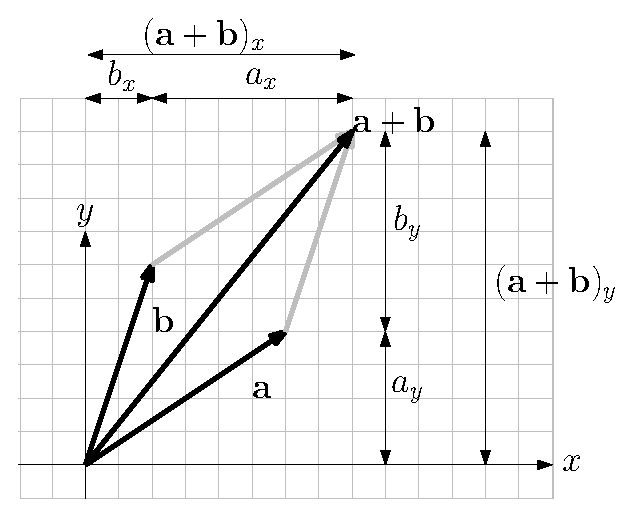
\includegraphics[width=8cm]{Math_vector/vectorAdd.eps}
\end{figure}
\end{frame}
%%%%%%%%%%%%%%%%%%%%%%%%%%%%%%%%%%%%%%%%%%%%%%%%%%%%%%%%%

%%%%%%%%%%%%%%%%%%%%%%%%%%%%%%%%%%%%%%%%%%%%%%%%%%%%%%%%%
\begin{frame}{벡터의 뺄셈}
$\mathbf v - \mathbf w = (v_x - w_x, v_y - w_y , v_z - w_z )$
\\

\begin{figure}
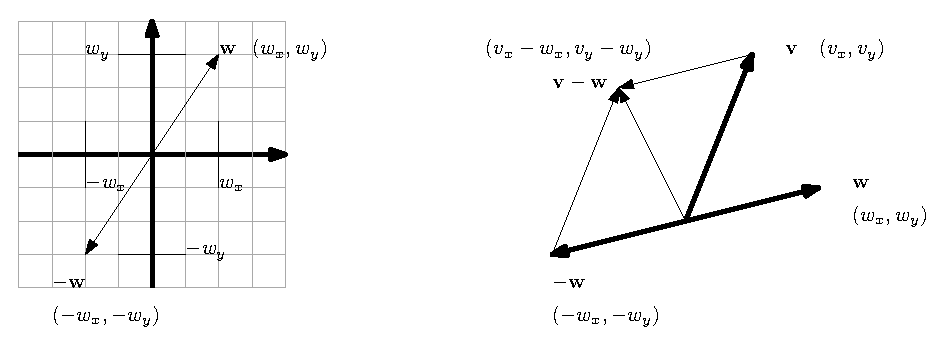
\includegraphics[width=12cm]{Math_vector/vectorSub.eps}
\end{figure}
\end{frame}
%%%%%%%%%%%%%%%%%%%%%%%%%%%%%%%%%%%%%%%%%%%%%%%%%%%%%%%%%

%%%%%%%%%%%%%%%%%%%%%%%%%%%%%%%%%%%%%%%%%%%%%%%%%%%%%%%%%
\begin{frame}{벡터에 스칼라 곱하기}

벡터는 크기만을 가진 스칼라와 곱할 수 있다. 어떤 스칼라 값 $s$가 있다고 하자, 이 스칼라 값과 벡터 $\mathbf v = (v_x , v_y, v_z)$를 곱한 $s \mathbf v$는 다음과 같다.
$$ s \mathbf v = (s v_x , s v_y , s v_z )$$
\end{frame}
%%%%%%%%%%%%%%%%%%%%%%%%%%%%%%%%%%%%%%%%%%%%%%%%%%%%%%%%%

%%%%%%%%%%%%%%%%%%%%%%%%%%%%%%%%%%%%%%%%%%%%%%%%%%%%%%%%%
\begin{frame}{벡터의 기본적인 연산 규칙}

\begin{eqnarray}
\mathbf a + \mathbf b = \mathbf b + \mathbf a \nonumber \\
(\mathbf a + \mathbf b) + \mathbf c = \mathbf a + (\mathbf b + \mathbf c) \nonumber \\
\mathbf a + \vec{0} = \vec{0} + \mathbf a = \mathbf a \nonumber \\
\mathbf a + (- \mathbf a) = \mathbf a - \mathbf a = \vec{0} \nonumber \\
(k+l) \mathbf a = k \mathbf a + l \mathbf a \nonumber \\
(kl) \mathbf a = k (l \mathbf a) \nonumber \\
1 \mathbf a = \mathbf a \nonumber \\
0 \mathbf a = \vec{0} \nonumber \\
(-1) \mathbf a = - \mathbf a \nonumber
\end{eqnarray}
\end{frame}
%%%%%%%%%%%%%%%%%%%%%%%%%%%%%%%%%%%%%%%%%%%%%%%%%%%%%%%%%

%%%%%%%%%%%%%%%%%%%%%%%%%%%%%%%%%%%%%%%%%%%%%%%%%%%%%%%%%
\begin{frame}{벡터의 스칼라 곱, 혹은 내적(dot product)}
\begin{itemize}
\item 내적
	\begin{itemize}
	\item 스칼라 곱(scalar product)라고도 부름 
	\item 두 개의 벡터를 피연산자(operand)로 하는 이항 연산(binary operator)로서 그 결과가 스칼라 값
	\item 두 벡터 $\mathbf a$와 $\mathbf b$의 내적은 $\mathbf a \cdot \mathbf b$로 표현
	\item 두 벡터가 이루는 사잇각이 $\theta$라고 하며, 내적의 크기는 다음과 같다.
		\begin{itemize}
		\item $\mathbf a \cdot \mathbf b = || \mathbf a || ||\mathbf b || \cos \theta$
		\end{itemize}
	\item 실제 계산 방법
		\begin{itemize}
		\item $\mathbf a , \mathbf b \in \mathbb R^n $
		\item $\mathbf a \cdot \mathbf b = a_1 b_1 + a_2 b_2 + \cdots + a_n b_n = \sum_{i=1}^n a_i b_i $
		\end{itemize}
	\end{itemize}
\end{itemize}

\end{frame}
%%%%%%%%%%%%%%%%%%%%%%%%%%%%%%%%%%%%%%%%%%%%%%%%%%%%%%%%%

%%%%%%%%%%%%%%%%%%%%%%%%%%%%%%%%%%%%%%%%%%%%%%%%%%%%%%%%%
\begin{frame}{벡터 내적의 의미}
\begin{figure}
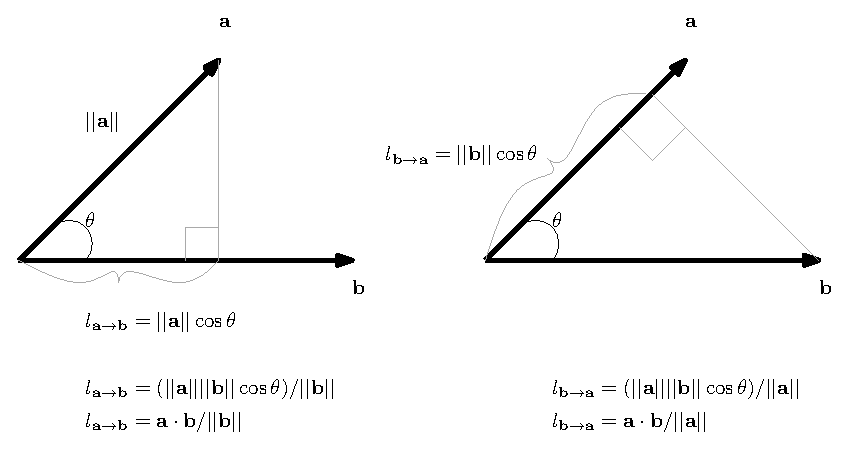
\includegraphics[width=12cm]{Math_vector/innerProduct.eps}
\end{figure}

\end{frame}
%%%%%%%%%%%%%%%%%%%%%%%%%%%%%%%%%%%%%%%%%%%%%%%%%%%%%%%%%


%%%%%%%%%%%%%%%%%%%%%%%%%%%%%%%%%%%%%%%%%%%%%%%%%%%%%%%%%
\begin{frame}{벡터 내적의 활용}
\begin{itemize}
\item 코사인 함수의 특성을 통해 간단히 얻어지는 사실
	\begin{itemize}
	\item $\theta = 0 \Rightarrow \cos \theta = 1 , \mathbf a \cdot \mathbf b = ||\mathbf a|| ||\mathbf b|| $
	\item $\theta = \pi / 2 \Rightarrow \cos \theta = 0, \mathbf a \cdot \mathbf b = 0 $
	\item $\mathbf a \cdot \mathbf a =  ||\mathbf a||^2$
	\end{itemize}
\end{itemize}


\begin{itemize}
\item 벡터를 이용하여 각도를 계산하거나 투영을 계산하는 데에 널리 사용
	\begin{itemize}
	\item $ \mathbf v \cdot \mathbf w  =  ||\mathbf v|| ||\mathbf w|| \cos \theta $
	\item $ \cos \theta = \frac{\mathbf v \cdot \mathbf w}{||\mathbf v||||\mathbf w||} $
	\item $ \theta  = \cos^{-1} \frac{\mathbf v \cdot \mathbf w}{||\mathbf v||||\mathbf w||} $
	\item $ \theta =  \cos^{-1}\frac{ v_x w_x + v_y w_y + v_z w_y}{\sqrt{v_x^2 + v_y^2 + v_z^2} \sqrt{w_x^2 + w_y^2 + w_z^2} }$
	\end{itemize} 
\end{itemize}

\end{frame}
%%%%%%%%%%%%%%%%%%%%%%%%%%%%%%%%%%%%%%%%%%%%%%%%%%%%%%%%%


%%%%%%%%%%%%%%%%%%%%%%%%%%%%%%%%%%%%%%%%%%%%%%%%%%%%%%%%%
\begin{frame}{벡터 내적의 활용}
\hrule

\noindent \colorbox{lightgray}{\begin{minipage}{6cm}예제\end{minipage}} 


\noindent 어떤 두 벡터가 각각 (3,2)와 (4,1)이라고 하자. 두 벡터가 이루는 각도를 구하라.

\noindent \colorbox{lightgray}{\begin{minipage}{6cm}정답\end{minipage}} 

\noindent 두 벡터를 각각 $\mathbf v$와 $\mathbf w$로 표현하자. 두 벡터의 내적 $\mathbf v \cdot \mathbf w$는 $3 \cdot 4 + 2 \cdot 1$, 즉 14이다.
각각의 길이는 $||\mathbf v|| = \sqrt{9+4} = \sqrt{13}$과 $||\mathbf w|| = \sqrt{16+1} = \sqrt{17}$이다.
따라서 두 벡터의 사이각은 다음과 같다.
$$\theta = \cos^{-1} \frac{14}{\sqrt{13} \sqrt{17}} = \cos^{-1} \frac{14}{\sqrt{221}} \simeq \cos^{-1} 0.94174191159484 \simeq 19.65 ^{\circ}$$

\hrule

\end{frame}
%%%%%%%%%%%%%%%%%%%%%%%%%%%%%%%%%%%%%%%%%%%%%%%%%%%%%%%%%


%%%%%%%%%%%%%%%%%%%%%%%%%%%%%%%%%%%%%%%%%%%%%%%%%%%%%%%%%
\begin{frame}{좌표축과 좌표 - 1/3 기본 의미}

\begin{itemize}
\item $\mathbf a  = (k, l)$로 표현된다는 것은 $xy$ 좌표계에서 기저벡터가 되는
$x$축 단위벡터를 $\mathbf u$와 $y$축 단위벡터를 $\mathbf v$를 다음과 같이 합성한 것
\end{itemize}

\begin{figure}
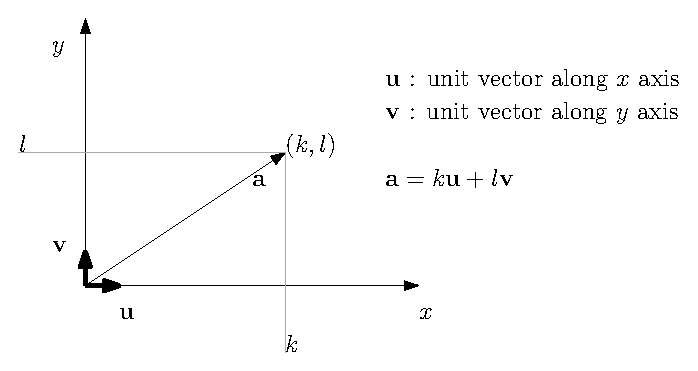
\includegraphics[width=10cm]{Math_vector/vectorComponents.eps}
\end{figure}

\end{frame}
%%%%%%%%%%%%%%%%%%%%%%%%%%%%%%%%%%%%%%%%%%%%%%%%%%%%%%%%%


%%%%%%%%%%%%%%%%%%%%%%%%%%%%%%%%%%%%%%%%%%%%%%%%%%%%%%%%%
\begin{frame}{좌표축과 좌표 - 2/3 새로운 축의 정의}

\begin{itemize}
\item 새로운 직교 좌표계를 고려해 보자. 여기서는 두 축이 $\mathbf u$와 $\mathbf v$
\item $\mathbf a$의 $\mathbf u$ 축 투영 길이 $\alpha$, $\mathbf v$ 축 투영 길이 $\beta$ 계산
\item 이 두 축을 기준으로 하는 좌표계에서는 $\mathbf a$가 $(\alpha, \beta)$의 좌표로 표현됨
\end{itemize}


\begin{figure}
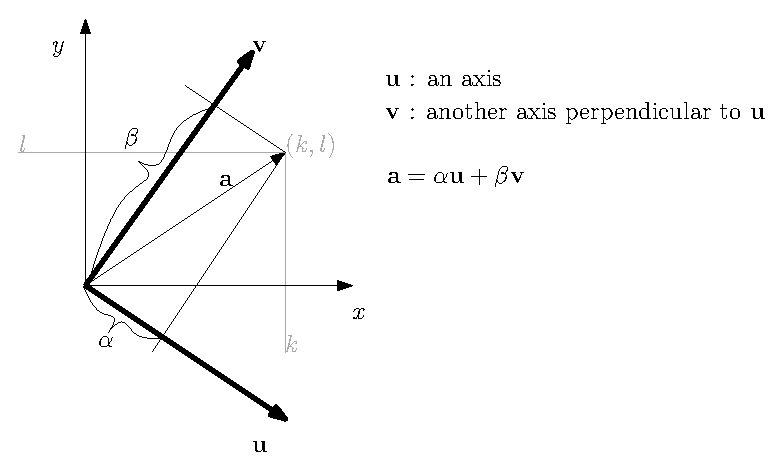
\includegraphics[width=10cm]{Math_vector/vectorComponentsArb.eps}
\end{figure}

\end{frame}
%%%%%%%%%%%%%%%%%%%%%%%%%%%%%%%%%%%%%%%%%%%%%%%%%%%%%%%%%

%%%%%%%%%%%%%%%%%%%%%%%%%%%%%%%%%%%%%%%%%%%%%%%%%%%%%%%%%
\begin{frame}{좌표축과 좌표 - 3/3 내적을 이용한 투영 길이 구하기}

\begin{itemize}
\item $\mathbf a$가 축 $\mathbf u$와 $\mathbf v$ 방향으로 가지는 길이 $\alpha$와 $\beta$는 어떻게 구하나
	\begin{itemize}
	\item 내적을 이용
	\item $\alpha$는 $\mathbf a$를 $\mathbf u$ 방향으로 투영한 그림자의 길이 =  $\mathbf a \cdot \mathbf u / || \mathbf u ||$
	\item 축은 단위 벡터로 표현하므로 $||\mathbf u||=1$. 따라서 $\alpha = \mathbf a \cdot \mathbf u$
	\item 비슷한 방법으로 $\beta = \mathbf a \cdot \mathbf v$
	\item $\mathbf u$와 $\mathbf v$를 축으로 하는 좌표계에서 $\mathbf a$는 $(\mathbf a \cdot \mathbf u, \mathbf a \cdot \mathbf v)$
	\end{itemize}
\end{itemize}

\begin{figure}
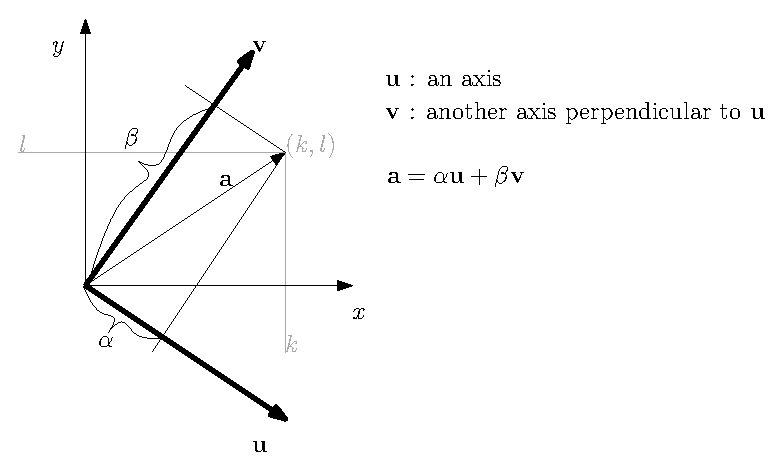
\includegraphics[width=6cm]{Math_vector/vectorComponentsArb.eps}
\end{figure}

\end{frame}
%%%%%%%%%%%%%%%%%%%%%%%%%%%%%%%%%%%%%%%%%%%%%%%%%%%%%%%%%


%%%%%%%%%%%%%%%%%%%%%%%%%%%%%%%%%%%%%%%%%%%%%%%%%%%%%%%%%
\begin{frame}{새로운 좌표축의 정의}

\hrule
\noindent \colorbox{lightgray}{\begin{minipage}{6cm}예제\end{minipage}} 


\noindent 그림처럼 어떤 벡터 $\mathbf a$가 (4,5)이고, 다른 벡터 $\mathbf b$는 (10,2)라고 하자.
이때 벡터 $\mathbf a$를 $\mathbf b$ 위에 수직방향으로 내린 그림자가 되는 벡터 $\mathbf a_{prj}$을 구하라.

\begin{figure}
    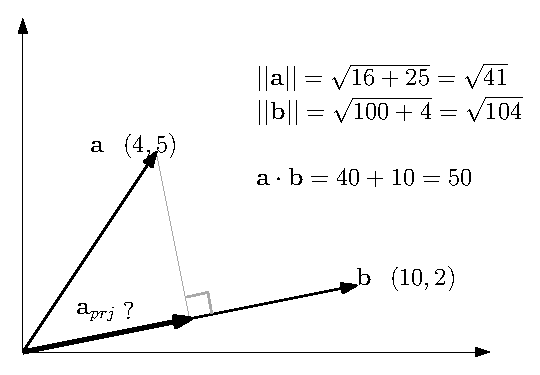
\includegraphics[width=4cm]{Math_vector/vecProjection.eps}
\end{figure}

\noindent \colorbox{lightgray}{\begin{minipage}{6cm}정답\end{minipage}} 

$$l = \mathbf a \cdot \mathbf b / || \mathbf b||$$
$$\mathbf a_{prj} = l \tilde{\mathbf b} = \frac{50}{104} (10,2)  \simeq  (4.8, 0.96) $$

\hrule

\end{frame}
%%%%%%%%%%%%%%%%%%%%%%%%%%%%%%%%%%%%%%%%%%%%%%%%%%%%%%%%%

%%%%%%%%%%%%%%%%%%%%%%%%%%%%%%%%%%%%%%%%%%%%%%%%%%%%%%%%%
\begin{frame}{벡터의 외적(外積) - 의미}

\begin{itemize}
\item 벡터의 외적(cross product)
	\begin{itemize}
	\item 벡터 곱(vector product): 두 벡터를 피연산자로 하는 이항연산으로 그 결과가 벡터
	\item 벡터를 곱해 행렬을 얻는 외적(outer product)과 용어의 혼동이 있음. 여기서는 결과가 벡터인 곱
	\end{itemize}
\item 표현
	\begin{itemize}
	\item 두 벡터 $\mathbf a$와 $\mathbf b$의 외적은 $\mathbf a \times \mathbf b$로 표현
	\item 그 결과는 벡터이므로 $k \mathbf n$ ($\mathbf n$은 $\mathbf a$와 $\mathbf b$에 동시에 수직인 단위벡터)
	\item 동시에 수직인 벡터는 두 개가 존재. 좌표계에 의해 결정됨.
	\end{itemize}
\end{itemize}

\begin{figure}
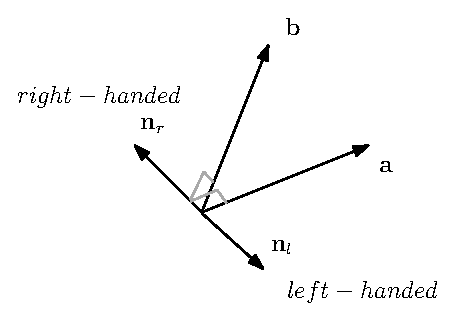
\includegraphics[width=5cm]{Math_vector/crossProductDir.eps}
\end{figure}

\end{frame}
%%%%%%%%%%%%%%%%%%%%%%%%%%%%%%%%%%%%%%%%%%%%%%%%%%%%%%%%%


%%%%%%%%%%%%%%%%%%%%%%%%%%%%%%%%%%%%%%%%%%%%%%%%%%%%%%%%%
\begin{frame}{벡터의 외적(外積) 의미의 수학적 표현}

\begin{itemize}
\item 두 벡터의 외적
	\begin{itemize}
	\item 외적의 크기 $k$
		\begin{itemize}
		\item 두 벡터의 크기와 사잇각의 사인(sine) 값에 비례
		\item $k = ||\mathbf a|| |\mathbf b|| \sin \theta$
		\end{itemize}
	\item 외적의 방향 $\mathbf n$
		\begin{itemize}
		\item $\mathbf n$: 두 벡터에 수직인 방향 벡터
		\end{itemize}
	\end{itemize}
\item 따라서 두 벡터의 외적은 다음과 같이 표현할 수 있다.
	\begin{itemize}
	\item $\mathbf a \times \mathbf b = ||\mathbf a|| |\mathbf b|| \sin \theta \mathbf n$
	\end{itemize}
\end{itemize}


\end{frame}
%%%%%%%%%%%%%%%%%%%%%%%%%%%%%%%%%%%%%%%%%%%%%%%%%%%%%%%%%

%%%%%%%%%%%%%%%%%%%%%%%%%%%%%%%%%%%%%%%%%%%%%%%%%%%%%%%%%
\begin{frame}{외적이 가진 의미}

\begin{itemize}
\item 외적을 표현하는 식 $\mathbf a \times \mathbf b = ||\mathbf a|| |\mathbf b|| \sin \theta \mathbf n$의 의미
	\begin{itemize}
	\item 외적은 두 벡터에 동시에 수직한 벡터
	\item 크기는 두 벡터가 수직일 때에 최대, 같은 방향이나 반대방향일 때 최소
	\item 외적의 크기는 벡터 $\mathbf a$와 $\mathbf b$의 끝점을 연결한 삼각형의 넓이 $S$에 비례
		\begin{itemize}
		\item $|| \mathbf a \times \mathbf b || = 2 S $
		\end{itemize}
		\end{itemize}
\end{itemize}


\begin{figure}
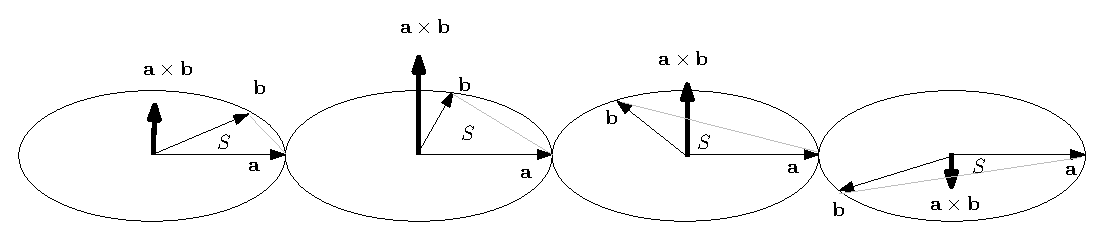
\includegraphics[width=12cm]{Math_vector/crossProductDirSize.eps}
\end{figure}

\end{frame}

%%%%%%%%%%%%%%%%%%%%%%%%%%%%%%%%%%%%%%%%%%%%%%%%%%%%%%%%%


%%%%%%%%%%%%%%%%%%%%%%%%%%%%%%%%%%%%%%%%%%%%%%%%%%%%%%%%%
\begin{frame}{외적의 계산}

\begin{itemize}
\item 3차원 벡터의 외적을 구하기
	\begin{itemize}
	\item $\mathbf a=(a_1, a_2, a_3), \mathbf b=(b_1, b_2, b_3)$
	\item 두 벡터의 외적: $\mathbf a \times \mathbf b = (a_2 b_3 - a_3 b_2, a_3 b_1 - a_1 b_3, a_1 b_2 - a_2 b_1)$
	\end{itemize}
\item ``행렬"을 이용한 곱셈으로 구하기
	\begin{itemize}
	\item ``반대칭(skew-symmetric 혹은 antisymmetric)" 행렬 이용
	\end{itemize}
\end{itemize}

\begin{eqnarray}
\mathbf A^* = \left ( 
\begin{array}{ccc}
0 & -a_3 & a_2 \\
a_3 & 0 & -a_1 \\
-a_2 & a_1 & 0 \nonumber
\end{array}
\right ) \nonumber
\end{eqnarray}

\begin{eqnarray}
\mathbf A^* \mathbf b = \left ( 
\begin{array}{ccc}
0 & -a_3 & a_2 \\
a_3 & 0 & -a_1 \\
-a_2 & a_1 & 0
\end{array}
\right ) \mathbf b
= (a_2 b_3 - a_3 b_2, a_3 b_1 - a_1 b_3, a_1 b_2 - a_2 b_1 ) \nonumber
\end{eqnarray}

\end{frame}

%%%%%%%%%%%%%%%%%%%%%%%%%%%%%%%%%%%%%%%%%%%%%%%%%%%%%%%%%


%%%%%%%%%%%%%%%%%%%%%%%%%%%%%%%%%%%%%%%%%%%%%%%%%%%%%%%%%
\begin{frame}{외적의 연산 법칙들}

\begin{eqnarray}\nonumber
\mathbf a \times \mathbf b = - \mathbf b \times \mathbf a \\ \nonumber
\mathbf a \times ( \mathbf b \times \mathbf c) = (\mathbf a \times \mathbf b) \times \mathbf c \\ \nonumber
(\mathbf a + \mathbf b ) \times \mathbf c = (\mathbf a \times \mathbf c) + (\mathbf b \times \mathbf c) \\ \nonumber
k(\mathbf a \times \mathbf b) = k \mathbf a \times \mathbf b = \mathbf a \times k \mathbf b \\ \nonumber
\mathbf a \times \vec{0} = \vec{0} \times \mathbf a = \vec{0} \\ \nonumber
\mathbf a \times \mathbf a = \vec{0} \\ \nonumber
\mathbf a \cdot (  \mathbf a \times \mathbf b) = \vec{0} \\ \nonumber
\mathbf b \cdot ( \mathbf a \times \mathbf b) = \vec{0}
\end{eqnarray}

\end{frame}
%%%%%%%%%%%%%%%%%%%%%%%%%%%%%%%%%%%%%%%%%%%%%%%%%%%%%%%%%


%%%%%%%%%%%%%%%%%%%%%%%%%%%%%%%%%%%%%%%%%%%%%%%%%%%%%%%%%
\begin{frame}{2차원 공간에서의 외적과 외적의 응용}

\begin{itemize}
\item 2차원 공간의 두 벡터 $\mathbf a=(a_x, a_y)$와 $\mathbf b=(b_x, b_y)$의 외적은?
	\begin{itemize}
	\item 그림의 회색 면은 2차원 공간의 일부
	\item 두 벡터 $\mathbf a$와 $\mathbf b$의 외적은 2차원 공간 밖에서 정의
	\item 축 $z$가 필요하며, 이 $z$ 축 성분으로만 표현
	\end{itemize}
\end{itemize}

\begin{figure}
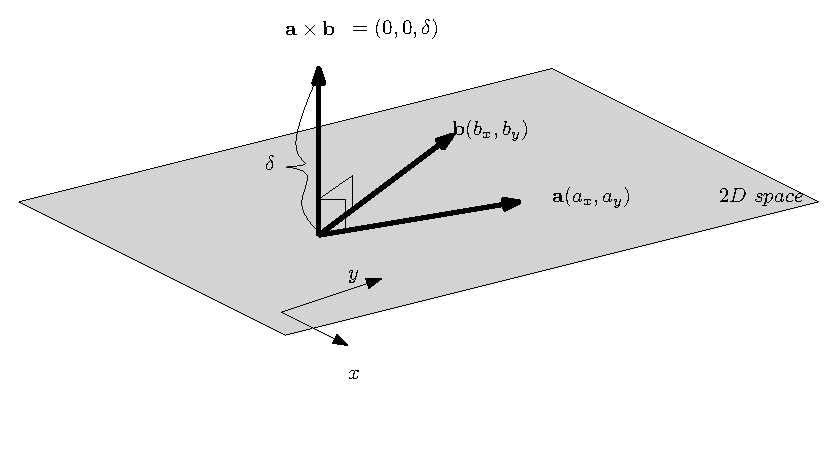
\includegraphics[width=12cm]{Math_vector/crossProduct2D.eps}
\end{figure}

\end{frame}
%%%%%%%%%%%%%%%%%%%%%%%%%%%%%%%%%%%%%%%%%%%%%%%%%%%%%%%%%


%%%%%%%%%%%%%%%%%%%%%%%%%%%%%%%%%%%%%%%%%%%%%%%%%%%%%%%%%
\begin{frame}{2차원 공간에서의 외적과 외적의 응용}
\begin{itemize}
\item 2차원 벡터의 외적이 2차원 공간 밖에 정의가 되고, 이것은 3차원 벡터라고 볼 수 있다.
\item 2차원 벡터 $\mathbf a = (a_x, a_y)$와 $\mathbf b= (b_x, b_y)$를 3차원 벡터로 가정
	\begin{itemize}
	\item $\mathbf a = (a_x , a_y, 0)$
	\item $\mathbf b = (b_x , b_y, 0)$
	\item $\mathbf a \times \mathbf b = (0, 0, a_x b_y - a_y b_x )$
	\end{itemize}
\end{itemize}

\begin{itemize}
\item $z$ 성분의 값으로 알 수 있는 것들  (이를 $\delta$라고 하자) 
	\begin{itemize}
	\item $\delta>0$인 경우는 $\mathbf b$가 $\mathbf a$의 진행 방향을 기준으로 왼쪽에 있음
	\item $\delta<0$인 경우는 오른쪽
	\item 절대값은 두 벡터 사이에 만들어지는 삼각형의 크기에 비례
	\end{itemize}
\end{itemize}

\end{frame}
%%%%%%%%%%%%%%%%%%%%%%%%%%%%%%%%%%%%%%%%%%%%%%%%%%%%%%%%%


%%%%%%%%%%%%%%%%%%%%%%%%%%%%%%%%%%%%%%%%%%%%%%%%%%%%%%%%%
\begin{frame}{삼각형 넓이 구하기}

\hrule
\noindent \colorbox{lightgray}{\begin{minipage}{6cm}예제\end{minipage}} 

\noindent 꼭지점 좌표가 (2,1), (8,4), (4,8)인 삼각형의 넓이 $S$를 구하라.

\noindent \colorbox{lightgray}{\begin{minipage}{6cm}정답\end{minipage}} 

{\small 꼭지점들을 각각 $\mathbf a, \mathbf b, \mathbf c$로 표현하자.
우리는 $\mathbf a$에서 $\mathbf b$로 가는 벡터를 구할 수 있고, $\mathbf u = (6,3)$가 된다.
비슷한 방식으로 $\mathbf a$에서 $\mathbf c$로 가는 벡터는 $\mathbf v = (2,7)$이다.
삼각형의 넓이는 이 두 벡터의 외적이 가지는 크기의 반이다.}

$$S = \frac{1}{2} ||\mathbf a \times \mathbf b || = \frac{6 \cdot 7 - 3 \cdot 2}{2} = 18$$

\begin{figure}
    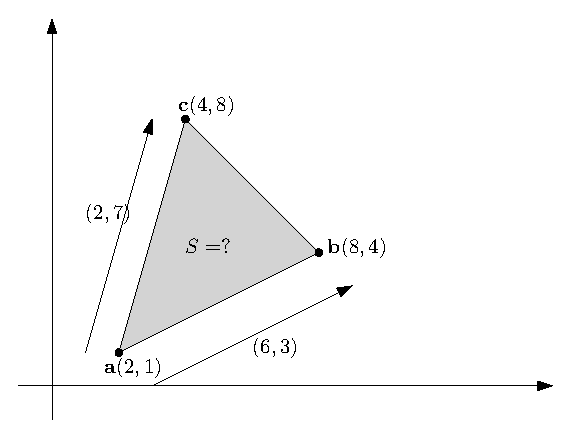
\includegraphics[width=4cm]{Math_vector/triangleArea.eps}
\end{figure}

\hrule

\end{frame}
%%%%%%%%%%%%%%%%%%%%%%%%%%%%%%%%%%%%%%%%%%%%%%%%%%%%%%%%%

%%%%%%%%%%%%%%%%%%%%%%%%%%%%%%%%%%%%%%%%%%%%%%%%%%%%%%%%%
\begin{frame}{외적과 평면}

\begin{itemize}
\item 외적의 또 다른 응용
	\begin{itemize}
	\item 평면 표현
		\begin{itemize}
		\item 평면은 그 평면 위의 삼각형으로 표현 가능 = 3 개의 점 = 9 개의 원소
		\item 좀 더 효율적인 방법 = 법선 벡터를 이용하기
		\item 법선벡터 = 평면이 바라보는 방향을 나타내는 벡터
		\item 법선벡터가 나타내는 것은 하나의 평면이 아니라 동일한 방향을 쳐다보는 모든 평면
		\item 평면의 표현 = (법선벡터, 평면이 지나는 점) : 6 개의 원소로 표현 가능
		\item 법선벡터 구하기: 벡터의 외적을 이용
		\end{itemize}
	\end{itemize}
\end{itemize}

\end{frame}


\end{document}


